% =====================================================================
%  c00 —— 标题页、译者说明、目录（Lead 独占）
%  对应原文 PDF p.1（标题 / 作者 / 图 1 / 课程说明 / 脚注）
% =====================================================================

\begin{titlepage}
\centering
\vspace*{2.2cm}

{\Large\bfseries 讲义与注记\\[0.4em]
Mirzakhani 的体积递推，以及研究\\[0.1em]
模空间 tautological 相交数的\\[0.1em]
Witten--Kontsevich 定理的途径\par}

\vspace{1.6cm}
{\large Scott A. Wolpert\par}

\vspace{2.2cm}
{\normalsize 中文译注本\par}
\vspace{0.3cm}
{\small 底本：arXiv:1108.0174v1 [math.DG]，2011 年 7 月 31 日\par}
{\small （原文标题页另印有日期 November 27, 2024，为 PDF 生成日期，非论文发表日期；\par}
{\small 原文作者的资助脚注已移入下文"短课程说明"。）\par}
{\small 38 页 ／ 11 图 ／ 15 条编号陈述 ／ 33 条参考文献\par}

\vfill
{\small 译者说明与全部译者批注见《译注汇总》；编译方法与已知限制见《README》。\par}
\end{titlepage}

% [原文 p.1] —— 标题页附注：本材料是 2011 年 Park City 数学研究所研究生暑期学校
%  "Riemann 曲面模空间" 短课程的讲稿；作者致谢 Brad Safnuk 协助备课与授课；
%  作者受 NSF DMS-1005852 部分资助。
\section*{短课程说明（原文 p.1）}
\addcontentsline{toc}{section}{短课程说明（原文 p.1）}

本材料曾于 2011 年 Park City 数学研究所（Park City Mathematics Institute）研究生暑期学校
"Riemann 曲面模空间"（Moduli Spaces of Riemann Surfaces）的一门短课程中讲授。
Brad Safnuk 协助了课程的准备与运行；作者谨此感谢他的帮助。
（原文脚注：作者部分受美国国家科学基金会资助（Partially supported），批准号 DMS-1005852。）

% [原文 p.1] 图 1
\begin{figure}[htbp]
\centering
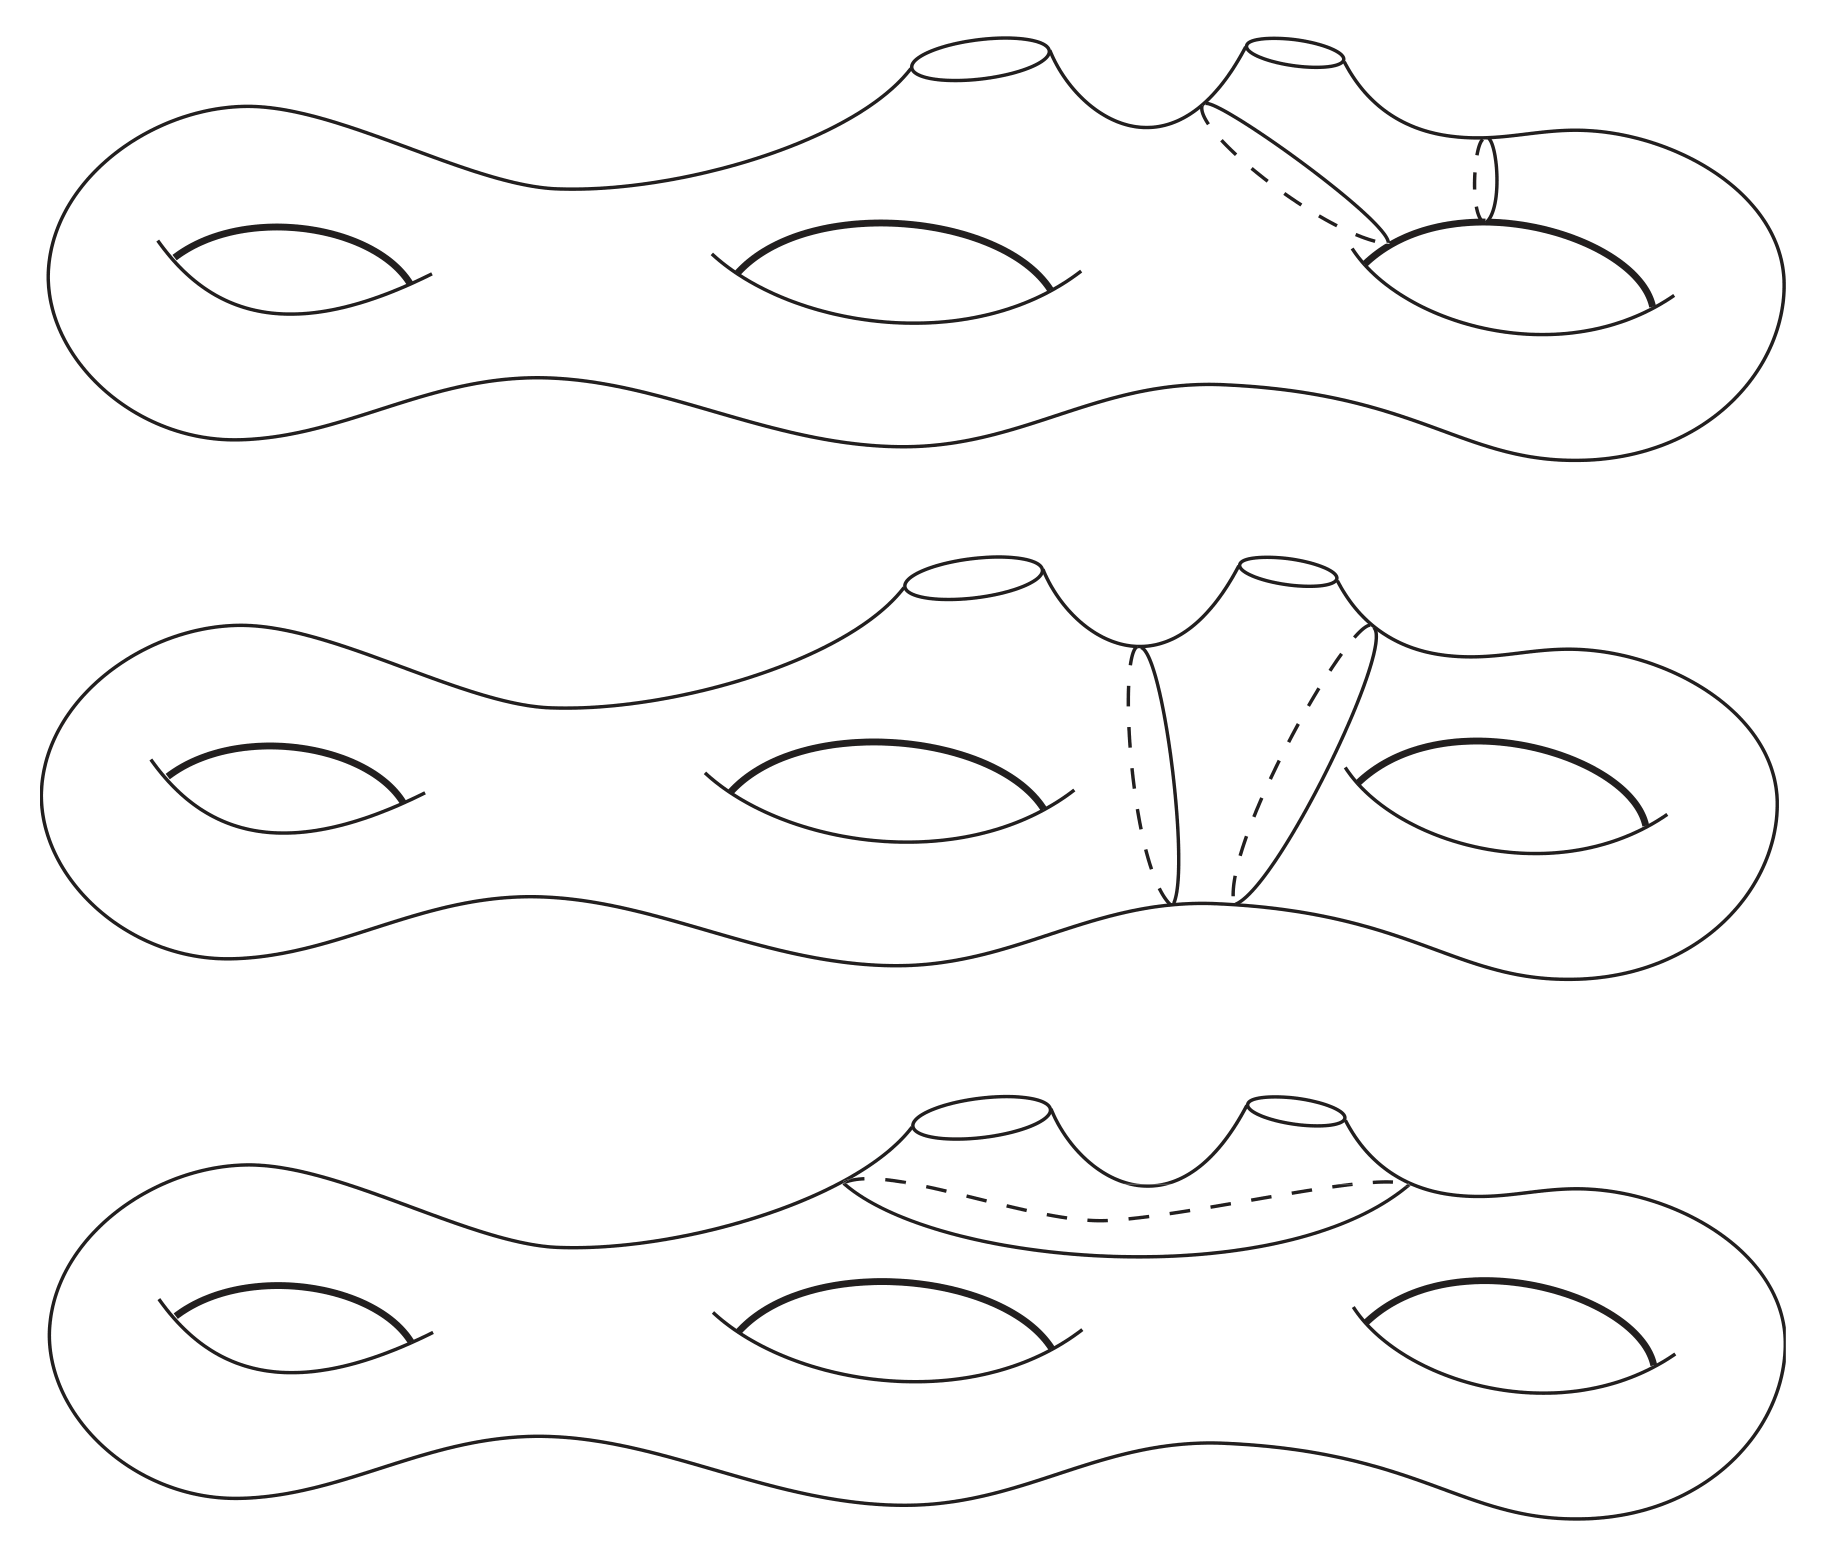
\includegraphics[width=0.62\textwidth]{fig01.png}
\figtitle{1}{长度恒等式所涉及的边界裤子构型。}
\end{figure}

% [Tutor Note: 图 1 画的是三条裤子（pants）在边界上按不同方式拼接得到的若干"边界裤子构型"，
%  与后文 §3 的长度恒等式 sum over pants 直接对应。读者若先记住"求和遍历所有嵌入的
%  β-裤子"，第 18--19 页的证明会顺畅得多。]

\vspace{1em}
\noindent\textbf{译者说明}\quad
（1）本译本以 2011 年 7 月 31 日 arXiv:1108.0174v1 为底本，全文 38 页。
底本的编号对象是 4 条编号公式（(1)--(4)）、15 条定理类陈述（Theorem 1--15，其中第 12 条为 Definition）
与 11 幅图，本译本逐一复刻其编号；其余公式底本未编号，译本同样不编号。

（2）正文严格照原文翻译，不放宽、不删节；凡解释性内容一律写入
\texttt{\% [Tutor Note: ...]} 注释，不进入排版。

（3）原文疑似的笔误照原样排，另行在批注中说明并给出正确形式（登记见 README）。

（4）参考文献保留英文原貌，逐条转录，未作翻译（学术惯例）。

\tableofcontents
\newpage
